\documentclass[11pt,a4paper]{article}

\usepackage[margin=22mm]{geometry}
\usepackage{amsmath,amssymb}
\usepackage{booktabs,array,longtable}
\usepackage{xcolor}
\usepackage{tikz}
\usetikzlibrary{arrows.meta,calc,positioning}
\usepackage[hidelinks]{hyperref}

\setlength{\parindent}{0pt}
\setlength{\parskip}{0.55em}
\renewcommand{\arraystretch}{1.18}

\newcommand{\Vd}{V_{\mathrm d}}
\newcommand{\rms}{\mathrm{rms}}
\newcommand{\avg}{\mathrm{avg}}
\newcommand{\pp}{\mathrm{pp}}
\newcommand{\unit}[1]{\,\mathrm{#1}}
\newcommand{\answerbox}[1]{\[\boxed{#1}\]}

\title{Power Electronics (UESTC3022)\\Homework Reference Solutions}
\author{Prepared from \texttt{materials/homework.pdf}}
\date{Academic Year 2025--2026, Semester II}

\begin{document}
\maketitle

\textbf{Note.} These are worked reference answers. Where the question or figure is ambiguous, the assumption used is stated explicitly. Numerical answers are rounded to a sensible number of significant figures.

\section*{Q1}

\subsection*{Q1(a): Average, RMS and form factor of the load current}

From Figure Q1-a, one period is read as $T=12\unit{ms}$ with current levels $+10\unit{A}$ and $-10\unit{A}$. One period can be divided as follows:
\[
\begin{array}{c|c}
\text{time interval} & \text{current waveform} \\
\hline
0\text{--}2\unit{ms} & 0\to +10\unit{A}\text{ ramp} \\
2\text{--}4\unit{ms} & +10\unit{A} \\
4\text{--}8\unit{ms} & +10\to -10\unit{A}\text{ ramp} \\
8\text{--}10\unit{ms} & -10\unit{A} \\
10\text{--}12\unit{ms} & -10\to 0\unit{A}\text{ ramp}.
\end{array}
\]

\textbf{(i) Average current.} The positive and negative areas are equal, so the signed average current is
\answerbox{I_{\avg}=0\unit{A}.}

\textbf{(ii) RMS current.} For a linear ramp from $0$ to $A$ lasting $\Delta t$, the contribution to $\int i^2dt$ is $\Delta t A^2/3$. For a linear ramp from $+A$ to $-A$ lasting $\Delta t$, the contribution is also $\Delta t A^2/3$. With $A=10\unit{A}$,
\begin{align*}
\int_0^T i^2(t)\,dt
&=\left(\frac{2}{3}+2+\frac{4}{3}+2+\frac{2}{3}\right)A^2 \unit{ms} \\
&=\frac{20}{3}A^2\unit{ms}.
\end{align*}
Therefore
\begin{align*}
I_{\rms}
&=\sqrt{\frac{1}{12}\frac{20}{3}A^2}
=A\sqrt{\frac{5}{9}}
=10\sqrt{\frac{5}{9}} \\
&=7.45\unit{A}.
\end{align*}
\answerbox{I_{\rms}\approx 7.45\unit{A}.}

\textbf{(iii) Form factor.} Since the signed average is zero, the useful form factor for an alternating waveform uses the rectified average value:
\[
I_{\avg,|\cdot|}=\frac{10+20+20+20+10}{12}=6.67\unit{A}.
\]
Thus
\[
\text{form factor}=\frac{I_{\rms}}{I_{\avg,|\cdot|}}
=\frac{7.45}{6.67}=1.12.
\]
\answerbox{\text{Form factor}\approx 1.12.}

\subsection*{Q1(b): Two-SCR bidirectional AC load controller}

\textbf{(i) Circuit.} Two SCRs are connected in anti-parallel and placed in series with the AC source and the resistive load. One SCR conducts during the positive half-cycle and the other SCR conducts during the negative half-cycle.

\begin{center}
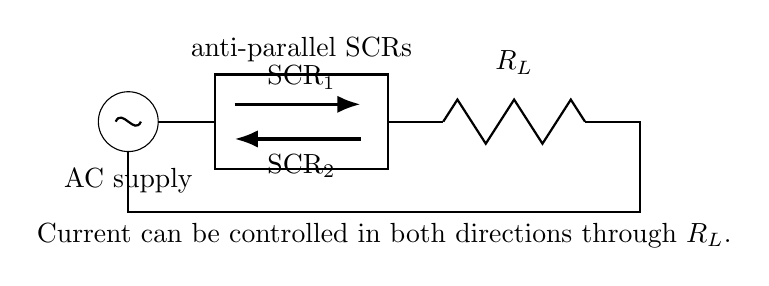
\begin{tikzpicture}[x=1cm,y=1cm,>=Latex]
  \draw (0,0) circle (0.38);
  \node at (0,-0.75) {AC supply};
  \draw[thick] (-0.16,0) .. controls (-0.08,0.18) and (0.08,-0.18) .. (0.16,0);
  \draw[thick] (0.38,0) -- (1.1,0);
  \draw[thick] (1.1,-0.6) rectangle (3.3,0.6);
  \draw[very thick,->] (1.35,0.22) -- (2.95,0.22);
  \draw[very thick,->] (2.95,-0.22) -- (1.35,-0.22);
  \node at (2.2,0.92) {anti-parallel SCRs};
  \node at (2.2,0.22) [above=2pt] {$\mathrm{SCR}_1$};
  \node at (2.2,-0.22) [below=2pt] {$\mathrm{SCR}_2$};
  \draw[thick] (3.3,0) -- (4.0,0);
  \draw[thick] (4.0,0) -- (4.18,0.28) -- (4.54,-0.28) -- (4.90,0.28) -- (5.26,-0.28) -- (5.62,0.28) -- (5.80,0);
  \node at (4.9,0.75) {$R_L$};
  \draw[thick] (5.8,0) -- (6.5,0) -- (6.5,-1.15) -- (0,-1.15) -- (0,-0.38);
  \node at (3.25,-1.45) {Current can be controlled in both directions through $R_L$.};
\end{tikzpicture}
\end{center}

\textbf{(ii) Phase-angle current sketches.} For a resistive load, the current follows the source sine wave after the relevant SCR is fired. A firing angle $\alpha>90^\circ$ gives less than half of the maximum power; a firing angle $\alpha<90^\circ$ gives more than half of the maximum power.

\begin{center}
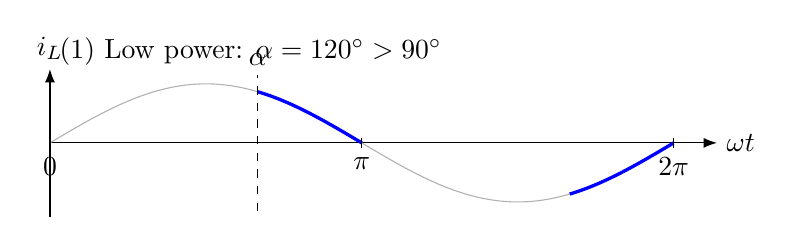
\begin{tikzpicture}[x=0.022cm,y=0.75cm,>=Latex]
  \node[anchor=west] at (0,1.55) {(1) Low power: $\alpha=120^\circ>90^\circ$};
  \draw[->] (0,0) -- (385,0) node[right] {$\omega t$};
  \draw[->] (0,-1.25) -- (0,1.25) node[above] {$i_L$};
  \draw[gray!60,domain=0:360,samples=120,variable=\a] plot ({\a},{sin(\a)});
  \draw[very thick,blue,domain=120:180,samples=50,variable=\a] plot ({\a},{sin(\a)});
  \draw[very thick,blue,domain=300:360,samples=50,variable=\a] plot ({\a},{sin(\a)});
  \draw[dashed] (120,-1.15)--(120,1.15) node[above] {$\alpha$};
  \foreach \x/\lab in {0/0,180/\pi,360/2\pi} {\draw (\x,0.08)--(\x,-0.08) node[below] {$\lab$};}
\end{tikzpicture}

\vspace{1em}

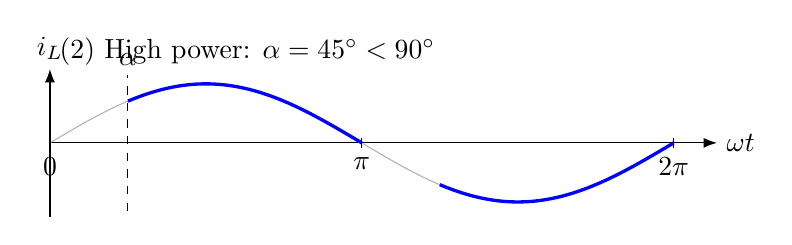
\begin{tikzpicture}[x=0.022cm,y=0.75cm,>=Latex]
  \node[anchor=west] at (0,1.55) {(2) High power: $\alpha=45^\circ<90^\circ$};
  \draw[->] (0,0) -- (385,0) node[right] {$\omega t$};
  \draw[->] (0,-1.25) -- (0,1.25) node[above] {$i_L$};
  \draw[gray!60,domain=0:360,samples=120,variable=\a] plot ({\a},{sin(\a)});
  \draw[very thick,blue,domain=45:180,samples=70,variable=\a] plot ({\a},{sin(\a)});
  \draw[very thick,blue,domain=225:360,samples=70,variable=\a] plot ({\a},{sin(\a)});
  \draw[dashed] (45,-1.15)--(45,1.15) node[above] {$\alpha$};
  \foreach \x/\lab in {0/0,180/\pi,360/2\pi} {\draw (\x,0.08)--(\x,-0.08) node[below] {$\lab$};}
\end{tikzpicture}
\end{center}

For reference, for a resistive load controlled by anti-parallel SCRs,
\[
\frac{P}{P_{\max}}=\frac{\pi-\alpha}{\pi}+\frac{\sin(2\alpha)}{2\pi},
\]
so $\alpha=90^\circ$ gives $P/P_{\max}=0.5$.

\subsection*{Q1(c): MOSFET advantages and disadvantages}

\textbf{Advantages:}
\begin{enumerate}
\item Voltage-controlled device with very high input impedance; gate-drive power is small.
\item Very fast switching because there is no minority-carrier storage in normal operation.
\item Low conduction loss at low and medium voltage ratings when $R_{\mathrm{DS(on)}}$ is small.
\item Easy to parallel because positive temperature coefficient of $R_{\mathrm{DS(on)}}$ helps current sharing.
\item Well suited to high-frequency switch-mode power supplies.
\end{enumerate}

\textbf{Disadvantages:}
\begin{enumerate}
\item $R_{\mathrm{DS(on)}}$ increases strongly with voltage rating, so high-voltage MOSFETs can have high conduction loss.
\item Gate oxide is sensitive to electrostatic discharge and excessive gate-source voltage.
\item The intrinsic body diode may have significant reverse-recovery loss in some applications.
\item Device capacitances cause switching loss and can make high-frequency gate driving difficult.
\item The device still needs careful thermal design at high current or high switching frequency.
\end{enumerate}

\subsection*{Q1(d): Thermal design of MOSFET and diode}

Given
\[
P_M=1.0\unit{W},\qquad P_D=2.0\unit{W},\qquad
\theta_{jc}=3^\circ\mathrm{C/W},\qquad \theta_{ca}=60^\circ\mathrm{C/W},
\]
\[
T_a=25^\circ\mathrm{C},\qquad T_{j,\max}=125^\circ\mathrm{C}.
\]

\textbf{(i) Without a heatsink.} The total junction-to-ambient thermal resistance is
\[
\theta_{ja}=\theta_{jc}+\theta_{ca}=3+60=63^\circ\mathrm{C/W}.
\]
For the MOSFET,
\[
T_{j,M}=25+1(63)=88^\circ\mathrm{C},
\]
which is safe. For the diode,
\[
T_{j,D}=25+2(63)=151^\circ\mathrm{C},
\]
which is above $125^\circ\mathrm{C}$ and is not safe.
\answerbox{\text{The MOSFET is safe without a heatsink, but the diode is not.}}

\textbf{(ii) Common heatsink.} The diode is most at risk because it dissipates the larger power. With both devices on the same heatsink, the sink is heated by
\[
P_{\mathrm{tot}}=1+2=3\unit{W}.
\]
Neglecting case-to-sink resistance because it is not specified,
\[
T_{j,D}=T_a+P_{\mathrm{tot}}\theta_{sa}+P_D\theta_{jc}.
\]
The requirement is
\[
125\ge 25+3\theta_{sa}+2(3),
\]
so
\[
3\theta_{sa}\le 94,
\qquad
\theta_{sa}\le 31.3^\circ\mathrm{C/W}.
\]
\answerbox{\text{Specify a common heatsink with }\theta_{sa}\le 31^\circ\mathrm{C/W}.}
If a non-negligible case-to-sink resistance is used in practice, the selected heatsink must have a lower $\theta_{sa}$ to compensate.

\subsection*{Q1(e): Centre-tapped full-wave rectifier}

The transformer ratio is interpreted as primary:total-secondary $=4:1$. Hence
\[
V_{s,\rms,\mathrm{total}}=\frac{80}{4}=20\unit{V_{rms}}.
\]

\textbf{(i) Circuit type.} This is a centre-tapped full-wave diode rectifier.

\textbf{(ii) Total peak secondary voltage.}
\[
V_{p(\mathrm{sec,total})}=20\sqrt{2}=28.3\unit{V}.
\]
\answerbox{V_{p(\mathrm{sec,total})}=28.3\unit{V}.}
Each half-secondary therefore has peak voltage
\[
V_{p(\mathrm{half})}=\frac{28.3}{2}=14.14\unit{V}.
\]

\textbf{(iii) Voltage across $R_L$.} One diode conducts per half-cycle, so the output is a full-wave rectified sine wave. The peak output voltage is approximately
\[
V_{R,\mathrm{peak}}=14.14-0.7=13.44\unit{V}.
\]

\begin{center}
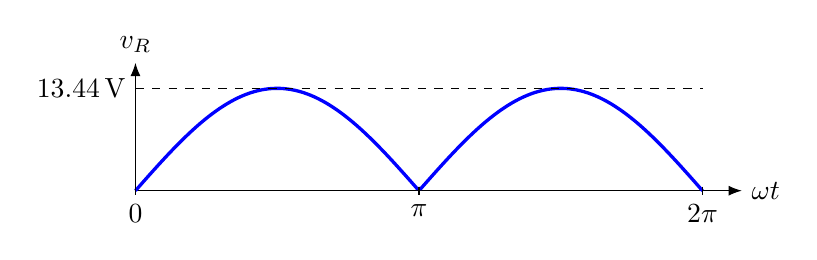
\begin{tikzpicture}[x=0.02cm,y=1.3cm,>=Latex]
  \draw[->] (0,0) -- (385,0) node[right] {$\omega t$};
  \draw[->] (0,0) -- (0,1.25) node[above] {$v_R$};
  \draw[very thick,blue,domain=0:360,samples=150,variable=\a] plot ({\a},{abs(sin(\a))});
  \draw[dashed] (0,1) -- (360,1);
  \node[left] at (0,1) {$13.44\unit{V}$};
  \foreach \x/\lab in {0/0,180/\pi,360/2\pi} {\draw (\x,0.04)--(\x,-0.04) node[below] {$\lab$};}
\end{tikzpicture}
\end{center}

\textbf{(iv) Peak current through each diode.}
\[
I_{D,\mathrm{peak}}=\frac{V_{R,\mathrm{peak}}}{R_L}
=\frac{13.44}{1000}=13.44\unit{mA}.
\]
\answerbox{I_{D,\mathrm{peak}}\approx 13.4\unit{mA}.}

\textbf{(v) Peak inverse voltage for each diode.} For a centre-tapped full-wave rectifier, the non-conducting diode sees approximately twice the half-secondary peak voltage. Including the conducting diode drop approximately,
\[
\mathrm{PIV}\approx 2(14.14)-0.7=27.6\unit{V}.
\]
The usual ideal-diode approximation is $2V_{p(\mathrm{half})}=28.3\unit{V}$.
\answerbox{\mathrm{PIV}\approx 28\unit{V}\text{ per diode}.}

\newpage
\section*{Q2}

\subsection*{Q2(a): Full-wave bridge rectifier}

The input is
\[
v_{ac}=100\sin(100\pi t),
\]
so
\[
V_m=100\unit{V},\qquad f=50\unit{Hz}.
\]
Because the rectifier is full-wave,
\[
f_{\mathrm{ripple}}=100\unit{Hz},\qquad T_{\mathrm{ripple}}=10\unit{ms}.
\]
The load resistance is $R_L=20\Omega$ and the smoothing capacitor is $C_s=10\unit{mF}=0.01\unit{F}$.

\textbf{(i) Ripple voltage and diode PIV.} The diode conduction angle is $30^\circ$. In a full-wave rectifier, each rectified cycle is $180^\circ$ or $10\unit{ms}$. Thus the conduction time is
\[
t_c=\frac{30^\circ}{180^\circ}(10\unit{ms})=1.667\unit{ms},
\]
and the capacitor discharge time is approximately
\[
\Delta t=10-1.667=8.333\unit{ms}.
\]
Using the standard linear discharge approximation,
\[
I_L\approx \frac{V_m}{R_L}=\frac{100}{20}=5\unit{A}.
\]
Therefore
\[
\Delta V_{R,\pp}\approx \frac{I_L\Delta t}{C_s}
=\frac{5(8.333\times10^{-3})}{0.01}=4.17\unit{V}.
\]
For a bridge rectifier with a capacitor output, the PIV of each diode is approximately the secondary peak voltage:
\[
\mathrm{PIV}\approx V_m=100\unit{V}.
\]
\answerbox{\Delta V_{R,\pp}\approx 4.17\unit{V},\qquad \mathrm{PIV}\approx 100\unit{V}.}

\textbf{(ii) Capacitor removed.} With $C_s$ removed, the load voltage is simply the full-wave rectified sine wave:
\[
v_R(t)=|100\sin(100\pi t)|.
\]
Its period is $10\unit{ms}$ and its peak value is $100\unit{V}$.

\begin{center}
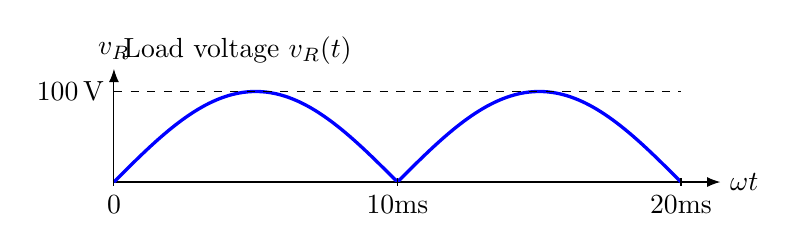
\begin{tikzpicture}[x=0.02cm,y=1.15cm,>=Latex]
  \node[anchor=west] at (0,1.45) {Load voltage $v_R(t)$};
  \draw[->] (0,0) -- (385,0) node[right] {$\omega t$};
  \draw[->] (0,0) -- (0,1.25) node[above] {$v_R$};
  \draw[very thick,blue,domain=0:360,samples=150,variable=\a] plot ({\a},{abs(sin(\a))});
  \draw[dashed] (0,1)--(360,1);
  \node[left] at (0,1) {$100\unit{V}$};
  \foreach \x/\lab in {0/0,180/10\mathrm{ms},360/20\mathrm{ms}} {\draw (\x,0.04)--(\x,-0.04) node[below] {$\lab$};}
\end{tikzpicture}

\vspace{1em}

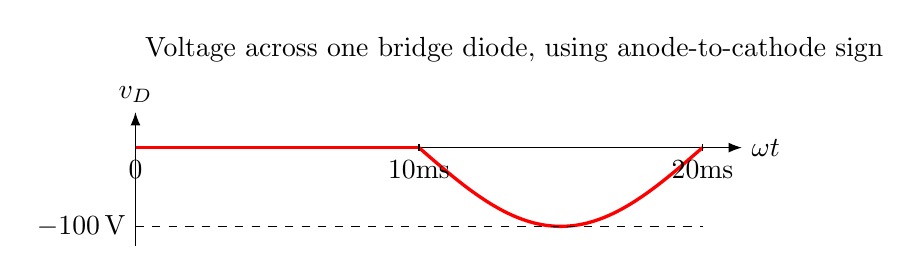
\begin{tikzpicture}[x=0.02cm,y=1.0cm,>=Latex]
  \node[anchor=west] at (0,1.25) {Voltage across one bridge diode, using anode-to-cathode sign};
  \draw[->] (0,0) -- (385,0) node[right] {$\omega t$};
  \draw[->] (0,-1.25) -- (0,0.45) node[above] {$v_D$};
  \draw[very thick,red] (0,0)--(180,0);
  \draw[very thick,red,domain=180:360,samples=80,variable=\a] plot ({\a},{sin(\a)});
  \draw[dashed] (0,-1)--(360,-1);
  \node[left] at (0,-1) {$-100\unit{V}$};
  \foreach \x/\lab in {0/0,180/10\mathrm{ms},360/20\mathrm{ms}} {\draw (\x,0.04)--(\x,-0.04) node[below] {$\lab$};}
\end{tikzpicture}
\end{center}

The RMS value of a full-wave rectified sine wave is the same as that of the original sine wave:
\[
V_{R,\rms}=\frac{V_m}{\sqrt{2}}=\frac{100}{\sqrt{2}}=70.7\unit{V}.
\]
\answerbox{V_{R,\rms}=70.7\unit{V}.}

\textbf{(iii) Capacitance for ripple not exceeding $1\unit{V_{pp}}$.} The question states that the capacitor may be assumed to supply the load current for each complete cycle of the rectified voltage, so use $\Delta t=10\unit{ms}$. With $I_L\approx 5\unit{A}$,
\[
C_s\approx \frac{I_L\Delta t}{\Delta V}
=\frac{5(10\times10^{-3})}{1}=0.05\unit{F}.
\]
\answerbox{C_s\approx 0.05\unit{F}=50\unit{mF}.}

\textbf{(iv) Effect of increasing only $C_s$.}
\begin{center}
\begin{tabular}{@{}ll@{}}
\toprule
Quantity & Effect of increasing $C_s$ \\
\midrule
Output ripple $\Delta V_R$ & decreases \\
Diode conduction angle & decreases; current pulses become narrower \\
Form factor of transformer current & increases, because the current becomes more peaky \\
Transformer VA rating & increases, because RMS current and peak current increase \\
\bottomrule
\end{tabular}
\end{center}

\textbf{(v) Advantages and disadvantages of the full bridge rectifier.}

\begin{center}
\begin{tabular}{@{}p{0.46\linewidth}p{0.46\linewidth}@{}}
\toprule
Advantages & Disadvantages \\
\midrule
Full-wave output, so ripple frequency is twice the supply frequency. & Two diodes conduct at a time, so there are two diode drops in a practical circuit. \\
No centre-tapped transformer is required. & Four diodes are required. \\
Better transformer utilisation than a centre-tapped full-wave rectifier. & With a large capacitor, the diode and transformer currents become narrow and high. \\
Each diode PIV is approximately only one secondary peak voltage. & Input current distortion, poor power factor and high inrush current can occur with capacitor smoothing. \\
\bottomrule
\end{tabular}
\end{center}

\subsection*{Q2(b): MOSFET thermal resistance}

Given
\[
\theta_{jc}=1.8^\circ\mathrm{C/W},\qquad
\theta_{cs}=0.6^\circ\mathrm{C/W},\qquad
T_a=50^\circ\mathrm{C},\qquad
T_{j,\max}=160^\circ\mathrm{C}.
\]

\textbf{(i) With $\theta_{sa}=7^\circ\mathrm{C/W}$.}
\[
\theta_{ja}=1.8+0.6+7=9.4^\circ\mathrm{C/W}.
\]
Thus
\[
P_{\max}=\frac{160-50}{9.4}=11.7\unit{W}.
\]
\answerbox{P_{\max}\approx 11.7\unit{W}.}

\textbf{(ii) Junction temperature at $20\unit{W}$.}
\[
T_j=50+20(9.4)=238^\circ\mathrm{C}.
\]
\answerbox{T_j=238^\circ\mathrm{C},\text{ which is not safe.}}

\textbf{(iii) Required heatsink thermal resistance for $20\unit{W}$.}
\[
160=50+20(1.8+0.6+\theta_{sa}).
\]
Therefore
\[
\theta_{sa}=\frac{110}{20}-2.4=5.5-2.4=3.1^\circ\mathrm{C/W}.
\]
\answerbox{\theta_{sa}\le 3.1^\circ\mathrm{C/W}.}

\newpage
\section*{Q3}

The problem concerns high-frequency voltage oscillation across a MOSFET caused by parasitic inductance and capacitance. The given values are
\[
L_p=20\unit{nH},\qquad C_p=500\unit{pF},\qquad f_s=200\unit{kHz},\qquad V_{\mathrm{bus}}=400\unit{V}.
\]

\subsection*{Q3(i): RC snubber design}

The approximate natural ringing frequency is
\[
f_0=\frac{1}{2\pi\sqrt{L_pC_p}}
=\frac{1}{2\pi\sqrt{(20\times10^{-9})(500\times10^{-12})}}
=50.3\unit{MHz}.
\]
The characteristic impedance of the parasitic resonance is
\[
Z_0=\sqrt{\frac{L_p}{C_p}}
=\sqrt{\frac{20\times10^{-9}}{500\times10^{-12}}}
=6.32\Omega.
\]

A common first-pass damping design for a series RC snubber across the MOSFET drain-source is therefore
\[
R_{\mathrm{snub}}\approx Z_0=6.32\Omega,
\qquad
C_{\mathrm{snub}}\approx 3C_p=1.5\unit{nF}.
\]
A practical strong-damping initial choice is therefore
\answerbox{R_{\mathrm{snub}}=6.2\Omega,\qquad C_{\mathrm{snub}}=1.5\unit{nF}.}
The capacitor should have a voltage rating above the $400\unit{V}$ bus, for example $630\unit{V}$ or $1\unit{kV}$ depending on the measured overshoot, and the resistor must be pulse-rated. The snubber should be placed physically very close to the MOSFET terminals to minimise added loop inductance.

\subsection*{Q3(ii): Snubber loss and portable-device compromise}

For a dissipative RC snubber whose capacitor is charged and discharged once per switching cycle, a conservative power estimate is
\[
P_{\mathrm{snub}}\approx C_{\mathrm{snub}}V_{\mathrm{bus}}^2f_s.
\]
Using the strong-damping design above,
\begin{align*}
P_{\mathrm{snub}}
&\approx (1.5\times10^{-9})(400)^2(200\times10^3) \\
&=48\unit{W}.
\end{align*}
Some texts use a one-transition estimate $P\approx \tfrac12 C_{\mathrm{snub}}V^2f_s$, which would still give $24\unit{W}$. In either case, this is far too high for most portable equipment: it wastes battery energy, increases temperature, and requires a large resistor.

A lower-loss compromise is to use a smaller snubber capacitor and accept partial damping, combined with layout and gate-drive improvements. For example, choose
\[
C_{\mathrm{snub}}=100\unit{pF}.
\]
The effective capacitance involved in the high-frequency ringing becomes approximately
\[
C_{\mathrm{eff}}=C_p+C_{\mathrm{snub}}=600\unit{pF},
\]
so a suitable damping resistor is
\[
R_{\mathrm{snub}}\approx\sqrt{\frac{L_p}{C_{\mathrm{eff}}}}
=\sqrt{\frac{20\times10^{-9}}{600\times10^{-12}}}
=5.77\Omega.
\]
A practical compromise selection is therefore
\answerbox{R_{\mathrm{snub}}=5.6\Omega,\qquad C_{\mathrm{snub}}=100\unit{pF}.}
The conservative loss estimate is then
\[
P_{\mathrm{snub}}\approx (100\times10^{-12})(400)^2(200\times10^3)=3.2\unit{W}.
\]
A one-transition estimate would be $1.6\unit{W}$. This is still significant in a portable device, but it is much more realistic than $24$--$48\unit{W}$. If measured oscillation remains unsafe, the capacitor can be increased, for example to $220\unit{pF}$, but the conservative loss would rise to about
\[
(220\times10^{-12})(400)^2(200\times10^3)=7.04\unit{W}.
\]
Thus the correct design process is not simply to maximise $C_{\mathrm{snub}}$; it is to use the smallest snubber that meets the measured voltage-stress and EMI requirements.

\subsection*{Q3(iii): Formal sources and holistic mitigation}

The snubber treats the symptom, namely ringing at the switch node. A more secure and robust design also reduces the root causes of the physical and electromagnetic risk.

\begin{longtable}{@{}p{0.30\linewidth}p{0.64\linewidth}@{}}
\toprule
Formal source & Holistic approach relevant to this problem \\
\midrule
Ott, \emph{Electromagnetic Compatibility Engineering} \cite{ott} & Treat EMI as a system problem. Reduce emissions at the source by minimising high-frequency loop area, controlling return current paths, using good grounding and bonding, and adding shielding or filtering where necessary. This directly reduces radiated EMI and therefore reduces the chance of information leakage from the converter. \\
Paul, \emph{Introduction to Electromagnetic Compatibility} \cite{paul} & Use the source--coupling-path--receiver model. Mitigation should reduce the source strength, interrupt the coupling path, and harden the receiver. For this converter, that means reducing switch-node $dv/dt$ and loop inductance, controlling common-mode current, filtering cables, and verifying emissions experimentally. \\
Erickson and Maksimovic, \emph{Fundamentals of Power Electronics} \cite{erickson} & Address converter-level causes of switching stress: device parasitics, layout inductance, gate-drive speed, diode reverse recovery, decoupling placement, and topology choice. Snubbers and clamps are useful, but lower parasitics and controlled switching transitions reduce the energy that must be dissipated in the snubber. \\
\bottomrule
\end{longtable}

A good final design should therefore combine the RC snubber with: compact drain-current loops, Kelvin-source gate return, local low-ESL DC-link capacitors, appropriate gate resistance or active gate control, suitable MOSFET voltage margin, short switch-node copper area, common-mode filtering or shielding where needed, and validation with oscilloscope and EMI measurements.

\newpage
\section*{Q4}

Assume the lower switches are driven complementarily to the upper switches, and dead time is neglected. The DC link is labelled $\Vd$, so if an upper switch is on, the corresponding phase pole is at $+\Vd/2$ with respect to the DC-link midpoint; if the upper switch is off, it is at $-\Vd/2$.

\subsection*{Q4(i): Key components and their functions}

\begin{center}
\begin{tabular}{@{}p{0.35\linewidth}p{0.58\linewidth}@{}}
\toprule
Component & Function \\
\midrule
DC supply / DC-link capacitor & Provides a stiff DC input voltage $\Vd$ and supplies pulsating inverter current. \\
Three inverter legs & Each phase leg contains an upper and lower switch; the leg connects the phase to either the positive or negative DC rail. \\
Power switches $T_{A\pm},T_{B\pm},T_{C\pm}$ & Chop the DC input to synthesise a three-phase AC output. \\
Anti-parallel diodes $D_{A\pm},D_{B\pm},D_{C\pm}$ & Provide freewheeling paths for inductive motor current when the switches commutate. \\
Gate-drive/control circuit & Generates the switching sequence and prevents shoot-through in each leg. \\
Three-phase load/motor & Receives the inverter line voltages and converts electrical power to mechanical power if it is a motor. \\
\bottomrule
\end{tabular}
\end{center}

\subsection*{Q4(ii): Line-voltage table}

The line voltages are
\[
v_{AB}=v_A-v_B,
\qquad
v_{BC}=v_B-v_C,
\qquad
v_{CA}=v_C-v_A.
\]
The switching table in the question gives the following results.

\begin{center}
\begin{tabular}{@{}c c c c c c c c c c@{}}
\toprule
Seq. & $T_{A+}$ & $T_{B+}$ & $T_{C+}$ & $v_A$ & $v_B$ & $v_C$ & $v_{AB}$ & $v_{BC}$ & $v_{CA}$ \\
\midrule
1 & On  & Off & On  & $+\Vd/2$ & $-\Vd/2$ & $+\Vd/2$ & $+\Vd$ & $-\Vd$ & $0$ \\
2 & On  & On  & Off & $+\Vd/2$ & $+\Vd/2$ & $-\Vd/2$ & $0$ & $+\Vd$ & $-\Vd$ \\
3 & Off & On  & Off & $-\Vd/2$ & $+\Vd/2$ & $-\Vd/2$ & $-\Vd$ & $+\Vd$ & $0$ \\
4 & Off & On  & On  & $-\Vd/2$ & $+\Vd/2$ & $+\Vd/2$ & $-\Vd$ & $0$ & $+\Vd$ \\
5 & Off & Off & On  & $-\Vd/2$ & $-\Vd/2$ & $+\Vd/2$ & $0$ & $-\Vd$ & $+\Vd$ \\
6 & On  & Off & Off & $+\Vd/2$ & $-\Vd/2$ & $-\Vd/2$ & $+\Vd$ & $0$ & $-\Vd$ \\
\bottomrule
\end{tabular}
\end{center}

\subsection*{Q4(iii): Line-voltage waveforms}

Each step lasts $60^\circ$, so over one electrical cycle the line voltages are:

\begin{center}
\begin{tabular}{@{}c c c c@{}}
\toprule
Electrical angle & $v_{AB}$ & $v_{BC}$ & $v_{CA}$ \\
\midrule
$0^\circ$--$60^\circ$ & $+\Vd$ & $-\Vd$ & $0$ \\
$60^\circ$--$120^\circ$ & $0$ & $+\Vd$ & $-\Vd$ \\
$120^\circ$--$180^\circ$ & $-\Vd$ & $+\Vd$ & $0$ \\
$180^\circ$--$240^\circ$ & $-\Vd$ & $0$ & $+\Vd$ \\
$240^\circ$--$300^\circ$ & $0$ & $-\Vd$ & $+\Vd$ \\
$300^\circ$--$360^\circ$ & $+\Vd$ & $0$ & $-\Vd$ \\
\bottomrule
\end{tabular}
\end{center}

\begin{center}
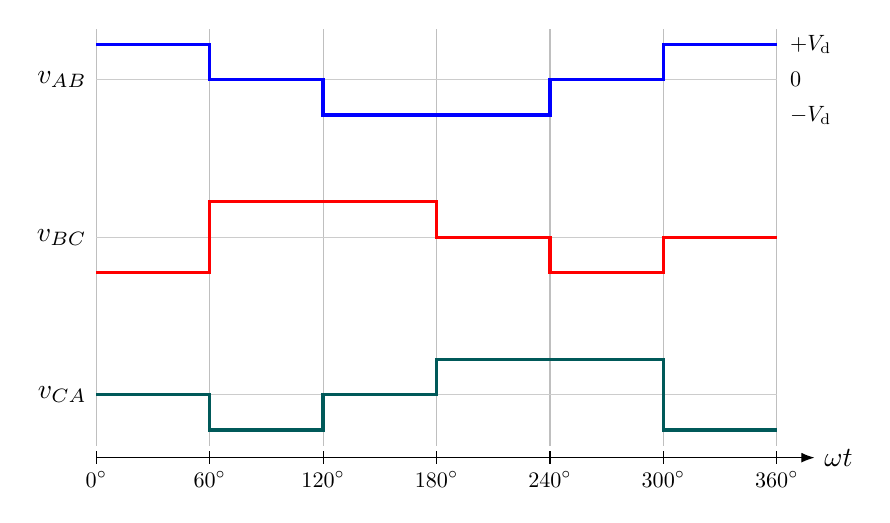
\begin{tikzpicture}[x=0.024cm,y=1cm,>=Latex]
  \def\s{0.45}
  \def\bA{2.6}
  \def\bB{0.6}
  \def\bC{-1.4}
  \draw[->] (0,-2.2) -- (380,-2.2) node[right] {$\omega t$};
  \foreach \x/\lab in {0/0^\circ,60/60^\circ,120/120^\circ,180/180^\circ,240/240^\circ,300/300^\circ,360/360^\circ} {
    \draw[gray!50] (\x,-2.05)--(\x,3.25);
    \draw (\x,-2.12)--(\x,-2.28) node[below,scale=0.8] {$\lab$};
  }
  \draw[gray!40] (0,\bA)--(360,\bA);
  \draw[gray!40] (0,\bB)--(360,\bB);
  \draw[gray!40] (0,\bC)--(360,\bC);
  \node[left] at (0,\bA) {$v_{AB}$};
  \node[left] at (0,\bB) {$v_{BC}$};
  \node[left] at (0,\bC) {$v_{CA}$};
  \draw[very thick,blue]
    (0,{\bA+\s}) -- (60,{\bA+\s}) -- (60,{\bA}) -- (120,{\bA}) --
    (120,{\bA-\s}) -- (180,{\bA-\s}) -- (240,{\bA-\s}) --
    (240,{\bA}) -- (300,{\bA}) -- (300,{\bA+\s}) -- (360,{\bA+\s});
  \draw[very thick,red]
    (0,{\bB-\s}) -- (60,{\bB-\s}) -- (60,{\bB+\s}) -- (120,{\bB+\s}) --
    (180,{\bB+\s}) -- (180,{\bB}) -- (240,{\bB}) --
    (240,{\bB-\s}) -- (300,{\bB-\s}) -- (300,{\bB}) -- (360,{\bB});
  \draw[very thick,teal!70!black]
    (0,{\bC}) -- (60,{\bC}) -- (60,{\bC-\s}) -- (120,{\bC-\s}) --
    (120,{\bC}) -- (180,{\bC}) -- (180,{\bC+\s}) -- (240,{\bC+\s}) --
    (300,{\bC+\s}) -- (300,{\bC-\s}) -- (360,{\bC-\s});
  \node[right,scale=0.8] at (363,{\bA+\s}) {$+\Vd$};
  \node[right,scale=0.8] at (363,{\bA}) {$0$};
  \node[right,scale=0.8] at (363,{\bA-\s}) {$-\Vd$};
\end{tikzpicture}
\end{center}

\subsection*{Q4(iv): Suitability for motor applications}

A normal six-step motor inverter should apply the six active switching states in a rotating order so that the three line-voltage fundamentals are balanced and separated by $120^\circ$. The sequence listed in the question uses the six active states, but the order is not the usual adjacent-vector order. In particular, the transition from sequence 1 $(101)$ to sequence 2 $(110)$ changes two phase legs at once and causes a larger voltage-vector jump.

Therefore, used exactly as listed, the waveform is not ideal for motor applications. It would give a distorted output with extra harmonic content and possible negative-sequence components, causing torque ripple, acoustic noise, extra heating and poorer speed control. A corrected six-step sequence such as
\[
100\to 110\to 010\to 011\to 001\to 101\to 100
\]
would be more appropriate for basic square-wave motor operation, although sinusoidal PWM or space-vector PWM would still be preferred for high-performance motor drives.

\subsection*{Q4(v): Effect of distorted inverter output on motor speed control and performance}

Distortion in the inverter output affects the motor in several ways:
\begin{enumerate}
\item Harmonic voltages create harmonic currents that do not contribute useful average torque.
\item Harmonic currents increase copper loss and iron loss, so the motor runs hotter and less efficiently.
\item Torque ripple increases, causing vibration and acoustic noise.
\item The fundamental voltage may be reduced or unbalanced, making speed and torque control less accurate.
\item High $dv/dt$ and voltage spikes can stress motor insulation and bearings.
\end{enumerate}
Overall, output distortion reduces efficiency, increases temperature and noise, and makes smooth speed control more difficult.

\begin{thebibliography}{9}
\bibitem{ott}
H. W. Ott, \emph{Electromagnetic Compatibility Engineering}. Hoboken, NJ: Wiley, 2009.

\bibitem{paul}
C. R. Paul, \emph{Introduction to Electromagnetic Compatibility}, 2nd ed. Hoboken, NJ: Wiley, 2006.

\bibitem{erickson}
R. W. Erickson and D. Maksimovic, \emph{Fundamentals of Power Electronics}, 2nd ed. New York: Kluwer Academic Publishers, 2001.
\end{thebibliography}

\end{document}
